\documentclass[11pt]{article}
\usepackage[utf8]{inputenc}
\usepackage[T1]{fontenc}
\usepackage{amsmath, amssymb}
\usepackage{booktabs}
\usepackage{siunitx}
\usepackage{graphicx}
\usepackage{hyperref}
\usepackage{geometry}
\geometry{margin=1in}

\title{Knowledge Distillation from a Vision Transformer Teacher\\
       to a MobileNetV2 Student on the Beans Leaf-Disease Dataset}
\author{}
\date{}

\begin{document}
\maketitle

% ============================================================
\section{Methodology}
% ============================================================

\subsection{Dataset}
We use the publicly available \emph{beans} leaf-disease dataset released by
the Makerere AI Lab \cite{mugalu2022makerere}.  It contains
1{,}295 RGB JPEG photographs of common bean (\emph{Phaseolus vulgaris}) leaves
collected in the field, originally at $500\times500$ pixels.  Each image is
labelled by an expert annotator with one of three classes:
\texttt{angular\_leaf\_spot} (a fungal disease caused by
\emph{Pseudocercospora griseola}), \texttt{bean\_rust} (caused by
\emph{Uromyces appendiculatus}), and \texttt{healthy}.  The official split
provides $1{,}034$ training, $133$ validation, and $128$ test images, with
classes nearly balanced in the training set ($345 / 348 / 341$, respectively).
All images are resized to $224\times224$.

\subsection{Teacher Model}
The teacher is the publicly released checkpoint
\texttt{merve/beans-vit-224}, a Vision Transformer with patch size
$16\times16$ (ViT-B/16) operating on $224\times224$ inputs
\cite{dosovitskiy2021vit}.  Its backbone has $12$ transformer encoder layers,
hidden size $768$, $12$ attention heads, and a $3072$-dimensional MLP per
block, for a total of \textbf{85.8\,M} parameters.  The backbone weights
originate from \texttt{google/vit-base-patch16-224-in21k}, a checkpoint
self-supervised pre-trained on \mbox{ImageNet-21k} ($\approx 14$\,M images,
$21{,}841$ classes).  The teacher model was fine-tuned on the beans
training set for $3$ epochs with the Adam optimizer~\cite{kingma2015adam}
(learning rate $5\times10^{-5}$, gradient accumulation giving an effective
batch size of $64$, linear schedule with warm-up ratio $0.1$), reaching a
test accuracy of $0.938$ on the beans test split.  We use the teacher only
for inference; its parameters are frozen during distillation.

\subsection{Student Model}
The student is a MobileNetV2 image classifier~\cite{sandler2018mobilenetv2}
with \textbf{2.23\,M} parameters, approximately $2.6\%$ of the teacher's
size.  We evaluate two initialization regimes.  Sections~\ref{subsec:test_results_baseline}
and~\ref{subsec:imagenet_ablation} compare random initialization against
ImageNet-1k pretrained weights from \texttt{google/mobilenet\_v2\_1.0\_224},
with the $3$-class head freshly initialized in both cases.

\subsection{Knowledge Distillation Strategy}
We follow the soft-target distillation formulation of
Hinton \emph{et~al.}~\cite{hinton2015distilling}.  Let $s\in\mathbb{R}^{C}$ and $t\in\mathbb{R}^{C}$
be the logits produced by the student and the (frozen) teacher for the same
input, $y$ the ground-truth one-hot label, $\sigma(\cdot)$ the softmax,
$T$ a temperature hyperparameter, and $\lambda\in[0,1]$ a mixing weight.
The student is trained to minimize
\begin{equation}
\mathcal{L}
\;=\;
(1-\lambda)\,\underbrace{\mathcal{L}_{\text{CE}}\bigl(s,\,y\bigr)}_{\text{hard targets}}
\;+\;
\lambda\,T^{2}\,
\underbrace{\mathrm{KL}\Bigl(\sigma\!\bigl(s/T\bigr)\;\Big\|\;\sigma\!\bigl(t/T\bigr)\Bigr)}_{\text{soft targets}}.
\label{eq:loss}
\end{equation}
The factor $T^{2}$ rescales the gradient magnitude of the soft term so it
remains comparable to the cross-entropy term as $T$ is varied.  We fix the
mixing weight to $\lambda=0.5$ and treat the temperature $T$ as the sole
distillation hyperparameter to be tuned.  A grid of values
$T\in\{1,2,3,4,5\}$ is explored with per-device batch size~$32$ (effective
batch $64$ under DistributedDataParallel across $2$ GPUs); for every
configuration the student is trained for $30$ epochs in fp16 mixed
precision~\cite{micikevicius2018mixed}.

\subsection{Non-uniform Saliency-based Sampling}
\label{subsec:saliency_sampler}

Distinguishing \texttt{angular\_leaf\_spot} from \texttt{bean\_rust} is a
fine-grained classification task: the discriminative cues are small
lesions occupying a small fraction of the leaf surface.  Uniformly resizing
each $500\times500$ image to the $224\times224$ input expected by both the
teacher and the student discards roughly $80\%$ of the original pixels and
may collapse a single lesion onto only a few output pixels.  To preserve
detail where it is most informative, we adopt the saliency-based sampling
layer of Recasens \emph{et~al.}~\cite{recasens2018learning} and place it
in front of the student.

\paragraph{Saliency network.}
A small convolutional network $f_{s}$ takes the uniformly downsampled
$224\times224$ view $I_{l}$ of the high-resolution input $I$ and produces a
single-channel saliency map $S=f_{s}(I_{l})$, normalized by a spatial softmax
so that $\sum_{x',y'} S(x',y')=1$.  In our setup $f_{s}$ consists of the first nine inverted-residual blocks
of \texttt{MobileNetV3-Small}~\cite{howard2019mobilenetv3} (pretrained on
ImageNet, $\approx 190$\,K parameters) followed by a $1\times1$
convolution that collapses the resulting feature map to a single
saliency channel.

\paragraph{Sampling approach.}
Treating $S(x',y')$ as an attractive mass on every input coordinate
$(x',y')$ and smoothing the attraction with a Gaussian kernel $k$, the
sampler computes the source coordinates $\bigl(u(x,y),v(x,y)\bigr)$ from
which each output pixel of the warped image $J$ is drawn:
\begin{align}
u(x,y) &= \frac{\displaystyle\sum_{x',y'} S(x',y')\,k\!\bigl((x,y),(x',y')\bigr)\,x'}
              {\displaystyle\sum_{x',y'} S(x',y')\,k\!\bigl((x,y),(x',y')\bigr)},
\label{eq:sampler_u}\\
v(x,y) &= \frac{\displaystyle\sum_{x',y'} S(x',y')\,k\!\bigl((x,y),(x',y')\bigr)\,y'}
              {\displaystyle\sum_{x',y'} S(x',y')\,k\!\bigl((x,y),(x',y')\bigr)}.
\label{eq:sampler_v}
\end{align}
The output $J(x,y)=I\!\bigl(u(x,y),v(x,y)\bigr)$ is then obtained by
bilinear interpolation on the high-resolution image $I$.  Both numerators
and the shared denominator in
Eqs.~\eqref{eq:sampler_u} and \eqref{eq:sampler_v} are computed by 2D
convolutions of $S$ and its coordinate-weighted variants with the kernel
$k$, so the layer is fully differentiable and can be trained end-to-end
with the task network.  The effect is to magnify regions where $S$ is large
and shrink regions where $S$ is small, while preserving the spatial topology
of $I$.

\paragraph{Training the sampler.}
Following \cite{recasens2018learning}, during the first $10$ epochs the
resampled image is briefly blurred via a random downsample-and-upsample
step to encourage $f_{s}$ to zoom into small regions; the blur is disabled
thereafter.  Optimization uses the SGD schedule prescribed
in~\cite{recasens2018learning} (momentum $0.9$, weight decay $10^{-4}$);
all other settings match Section~\ref{subsec:imagenet_ablation}.

% ============================================================
\section{Results}
% ============================================================

\subsection{Temperature finetuning (validation set)}
Table~\ref{tab:temperature_sweep} reports, for every temperature
$T\in\{1,2,3,4,5\}$, the best validation accuracy obtained during $30$
epochs of training.  The best configuration is $T=1$, reaching $0.7744$ on
validation at epoch~$26$.

\begin{table}[h]
\centering
\caption{Best validation accuracy on the beans validation set ($N{=}133$)
across the temperature grid.  All other hyperparameters are held fixed:
$\lambda{=}0.5$, per-device batch size $32$ (effective batch $64$ across
$2$ GPUs), $30$ epochs, AdamW~\cite{loshchilov2019adamw} with $\text{lr}=5\times10^{-5}$, fp16, seed
$42$.  The best row is shown in bold.}
\label{tab:temperature_sweep}
\begin{tabular}{c S[table-format=1.4] c}
\toprule
\textbf{Temperature $T$} & {\textbf{Best val accuracy}} & \textbf{Best epoch} \\
\midrule
1 & {\textbf{0.7744}} & 26 \\
2 & 0.6842 & 14 \\
3 & 0.7218 & 26 \\
4 & 0.7293 & 14 \\
5 & 0.7594 & 14 \\
\bottomrule
\end{tabular}
\end{table}

\subsection{Test-set comparison of distilled student, baseline, and teacher}
\label{subsec:test_results_baseline}
Using the best configuration from Table~\ref{tab:temperature_sweep} we
re-evaluate the student on the held-out test split.  As a no-distillation
control, we train the same MobileNetV2 architecture from scratch on the same
data with identical hyperparameters but with the cross-entropy term only
($\lambda{=}0$, equivalent to dropping the soft-target loss in
Eq.~\eqref{eq:loss}).  As an upper bound, we also report the frozen teacher
evaluated on the test split.  Results are summarized in
Table~\ref{tab:test_results}.

\begin{table}[h]
\centering
\caption{Test-set performance ($N{=}128$) of the three models: the
no-distillation baseline (MobileNetV2 trained from scratch with plain
cross-entropy), the distilled student trained with the best temperature
($T{=}1$, $\lambda{=}0.5$), and the ViT-B/16 teacher (inference only).
Initialization: $\dagger$~random (from scratch).}
\label{tab:test_results}
\begin{tabular}{l c c c c}
\toprule
\textbf{Model} & \textbf{Distill} & \textbf{Params} & \textbf{Test accuracy} & \textbf{Test macro-F1} \\
\midrule
Student$^{\dagger}$         &              & 2.23\,M  & 0.6094 & 0.6057 \\
Student$^{\dagger}$         & \checkmark   & 2.23\,M  & \textbf{0.7188} & \textbf{0.7202} \\
Teacher (ViT-B/16)          & ---          & 85.8\,M  & 0.9375 & 0.9379 \\
\bottomrule
\end{tabular}
\end{table}

Distillation lifts the same student architecture by $+0.109$ in test
accuracy and $+0.115$ in macro-F1 over the no-distillation baseline,
narrowing the accuracy gap to the much larger ViT teacher from $0.328$
to $0.219$.

\subsection{Ablation: ImageNet-pretrained student initialization}
\label{subsec:imagenet_ablation}
The runs above initialize the student randomly.  We repeat the temperature
sweep and the test-set comparison after replacing the random initialization
with the ImageNet-1k MobileNetV2 checkpoint
\texttt{google/mobilenet\_v2\_1.0\_224}~\cite{deng2009imagenet}; only the
$3$-class head is freshly initialized, and all other hyperparameters are
unchanged.  Every temperature now exceeds $0.95$ on validation.  Re-evaluating each
sweep checkpoint on the test split yields $0.9219$ at $T{=}1$, $0.8594$
at $T{=}2$, $0.8906$ at $T{=}3$, $0.8906$ at $T{=}4$, and $0.8672$ at
$T{=}5$.  Validation-best and test-best therefore disagree (the small
validation set, $N{=}133$, makes single-seed best-by-validation selection
unstable), and we report the test-best operating point ($T{=}1$) for the
head-to-head comparison in Table~\ref{tab:test_results_imagenet}.

\begin{table}[h]
\centering
\caption{Test-set performance ($N{=}128$) under ImageNet-1k student
initialization: the no-distillation baseline, the distilled student
($T{=}1$, $\lambda{=}0.5$), and the ViT-B/16 teacher (inference only).
Initialization: $\star$~ImageNet-1k pretrained.}
\label{tab:test_results_imagenet}
\begin{tabular}{l c c c c}
\toprule
\textbf{Model} & \textbf{Distill} & \textbf{Params} & \textbf{Test accuracy} & \textbf{Test macro-F1} \\
\midrule
Student$^{\star}$         &             & 2.23\,M & 0.8984 & 0.8992 \\
Student$^{\star}$         & \checkmark  & 2.23\,M & \textbf{0.9219} & \textbf{0.9224} \\
Teacher (ViT-B/16)        & ---         & 85.8\,M & 0.9375 & 0.9379 \\
\bottomrule
\end{tabular}
\end{table}

ImageNet initialization alone improves the no-distillation MobileNetV2
from $0.6094$ to $0.8984$ test accuracy ($+0.294$ macro-F1), closing
about $88\%$ of the baseline-to-teacher gap from
Table~\ref{tab:test_results}.  Adding distillation on top of the
ImageNet-initialized student then yields a further $+0.024$ accuracy and
$+0.023$ macro-F1, reaching $0.9219$ test accuracy, only $0.016$ below
the teacher.  Most of the headline gain in
Table~\ref{tab:test_results} therefore reflects the absence of any visual
prior in the random-init student rather than a property of distillation
itself; once the student carries an ImageNet prior, the soft-target
signal contributes a smaller marginal improvement.

\subsection{Adding the saliency sampler}
\label{subsec:sampler_results}
We re-run the best ImageNet-initialized configuration of
Section~\ref{subsec:imagenet_ablation} ($T{=}1$, $\lambda{=}0.5$) with the
saliency sampler of Section~\ref{subsec:saliency_sampler} placed in front
of the student.  The student now sees the warped $224\times224$ image
$J=g(I,S)$ rather than a uniform downsample of the $500\times500$ input;
the teacher continues to see the uniform $224\times224$ view it was
trained on.  As a control we also train an identical sampler-equipped
student without distillation ($\lambda=0$).
Table~\ref{tab:test_results_sampler} reports the test set performance.

\begin{table}[h]
\centering
\caption{Test set performance ($N{=}128$) of the ImageNet-initialized
MobileNetV2 student equipped with the saliency sampler, with and without
knowledge distillation.  The teacher upper bound and two prior reports on
the same beans dataset are listed for context.  The sampler adds the
truncated MobileNetV3-Small saliency network ($\approx 0.19$\,M
parameters) to the deployed model.  $^{\ddagger}$\,Abed
\emph{et~al.}~\cite{abed2021modern} use a 60/20/20 split (test
$N{\approx}259$) instead of the official 1{,}034/133/128 partition; macro
F1 not reported for the multi-class task in that work.}
\label{tab:test_results_sampler}
\begin{tabular}{l c c c c c}
\toprule
\textbf{Model} & \textbf{Sampler} & \textbf{Distill} & \textbf{Params} & \textbf{Test accuracy} & \textbf{Test macro-F1} \\
\midrule
Student$^{\star}$ (ours)    &              & \checkmark  & 2.23\,M             & 0.9219          & 0.9224          \\
Student$^{\star}$ (ours)    & \checkmark   &             & 2.23\,M $+$ 0.19\,M & 0.8984          & 0.8984          \\
Student$^{\star}$ (ours)    & \checkmark   & \checkmark  & 2.23\,M $+$ 0.19\,M & \textbf{0.9766} & \textbf{0.9767} \\
\midrule
MobileNetV2~\cite{elfatimi2022beans}        & ---  & --- & 2.23\,M  & 0.9297     & 0.9294 \\
DenseNet121$^{\ddagger}$~\cite{abed2021modern} & --- & --- & 8.0\,M   & 0.9102     & ---    \\
\midrule
Teacher (ViT-B/16)                          & ---  & --- & 85.8\,M  & 0.9375     & 0.9379 \\
\bottomrule
\end{tabular}
\end{table}

Both sampler-equipped runs reach the same best validation accuracy
($0.9925$, one validation error out of $133$), yet diverge by $+0.078$
test accuracy and $+0.078$ macro-F1 in favour of the distilled variant.
This isolates the role of the soft-target signal once the sampler has
already preserved the relevant fine-grained cues: the KD student exceeds
the ViT-B/16 teacher by $+0.039$ test accuracy ($+0.039$ macro-F1) with
about $2.8\%$ of the teacher's parameter count, while the no-KD ablation
falls $0.039$ short of the teacher despite the same architecture and
training data.

Figure~\ref{fig:sampler_qualitative} shows the qualitative behaviour of
the trained sampler on five representative test images.  For each image,
from left to right we display the original $500\times500$ input, the
$31\times31$ saliency map produced by $f_{s}$, the deformation grid
$g(\cdot,S)$ in the output coordinate frame (cells appear larger where
the warp magnifies the input), and the resulting $224\times224$ sampled
image $J$ that is fed to the student.  The saliency network consistently
discovers small lesion-like regions and the sampler concentrates output
pixels around them, in line with the fine-grained motivation of
Section~\ref{subsec:saliency_sampler}.

\begin{figure}[h]
\centering
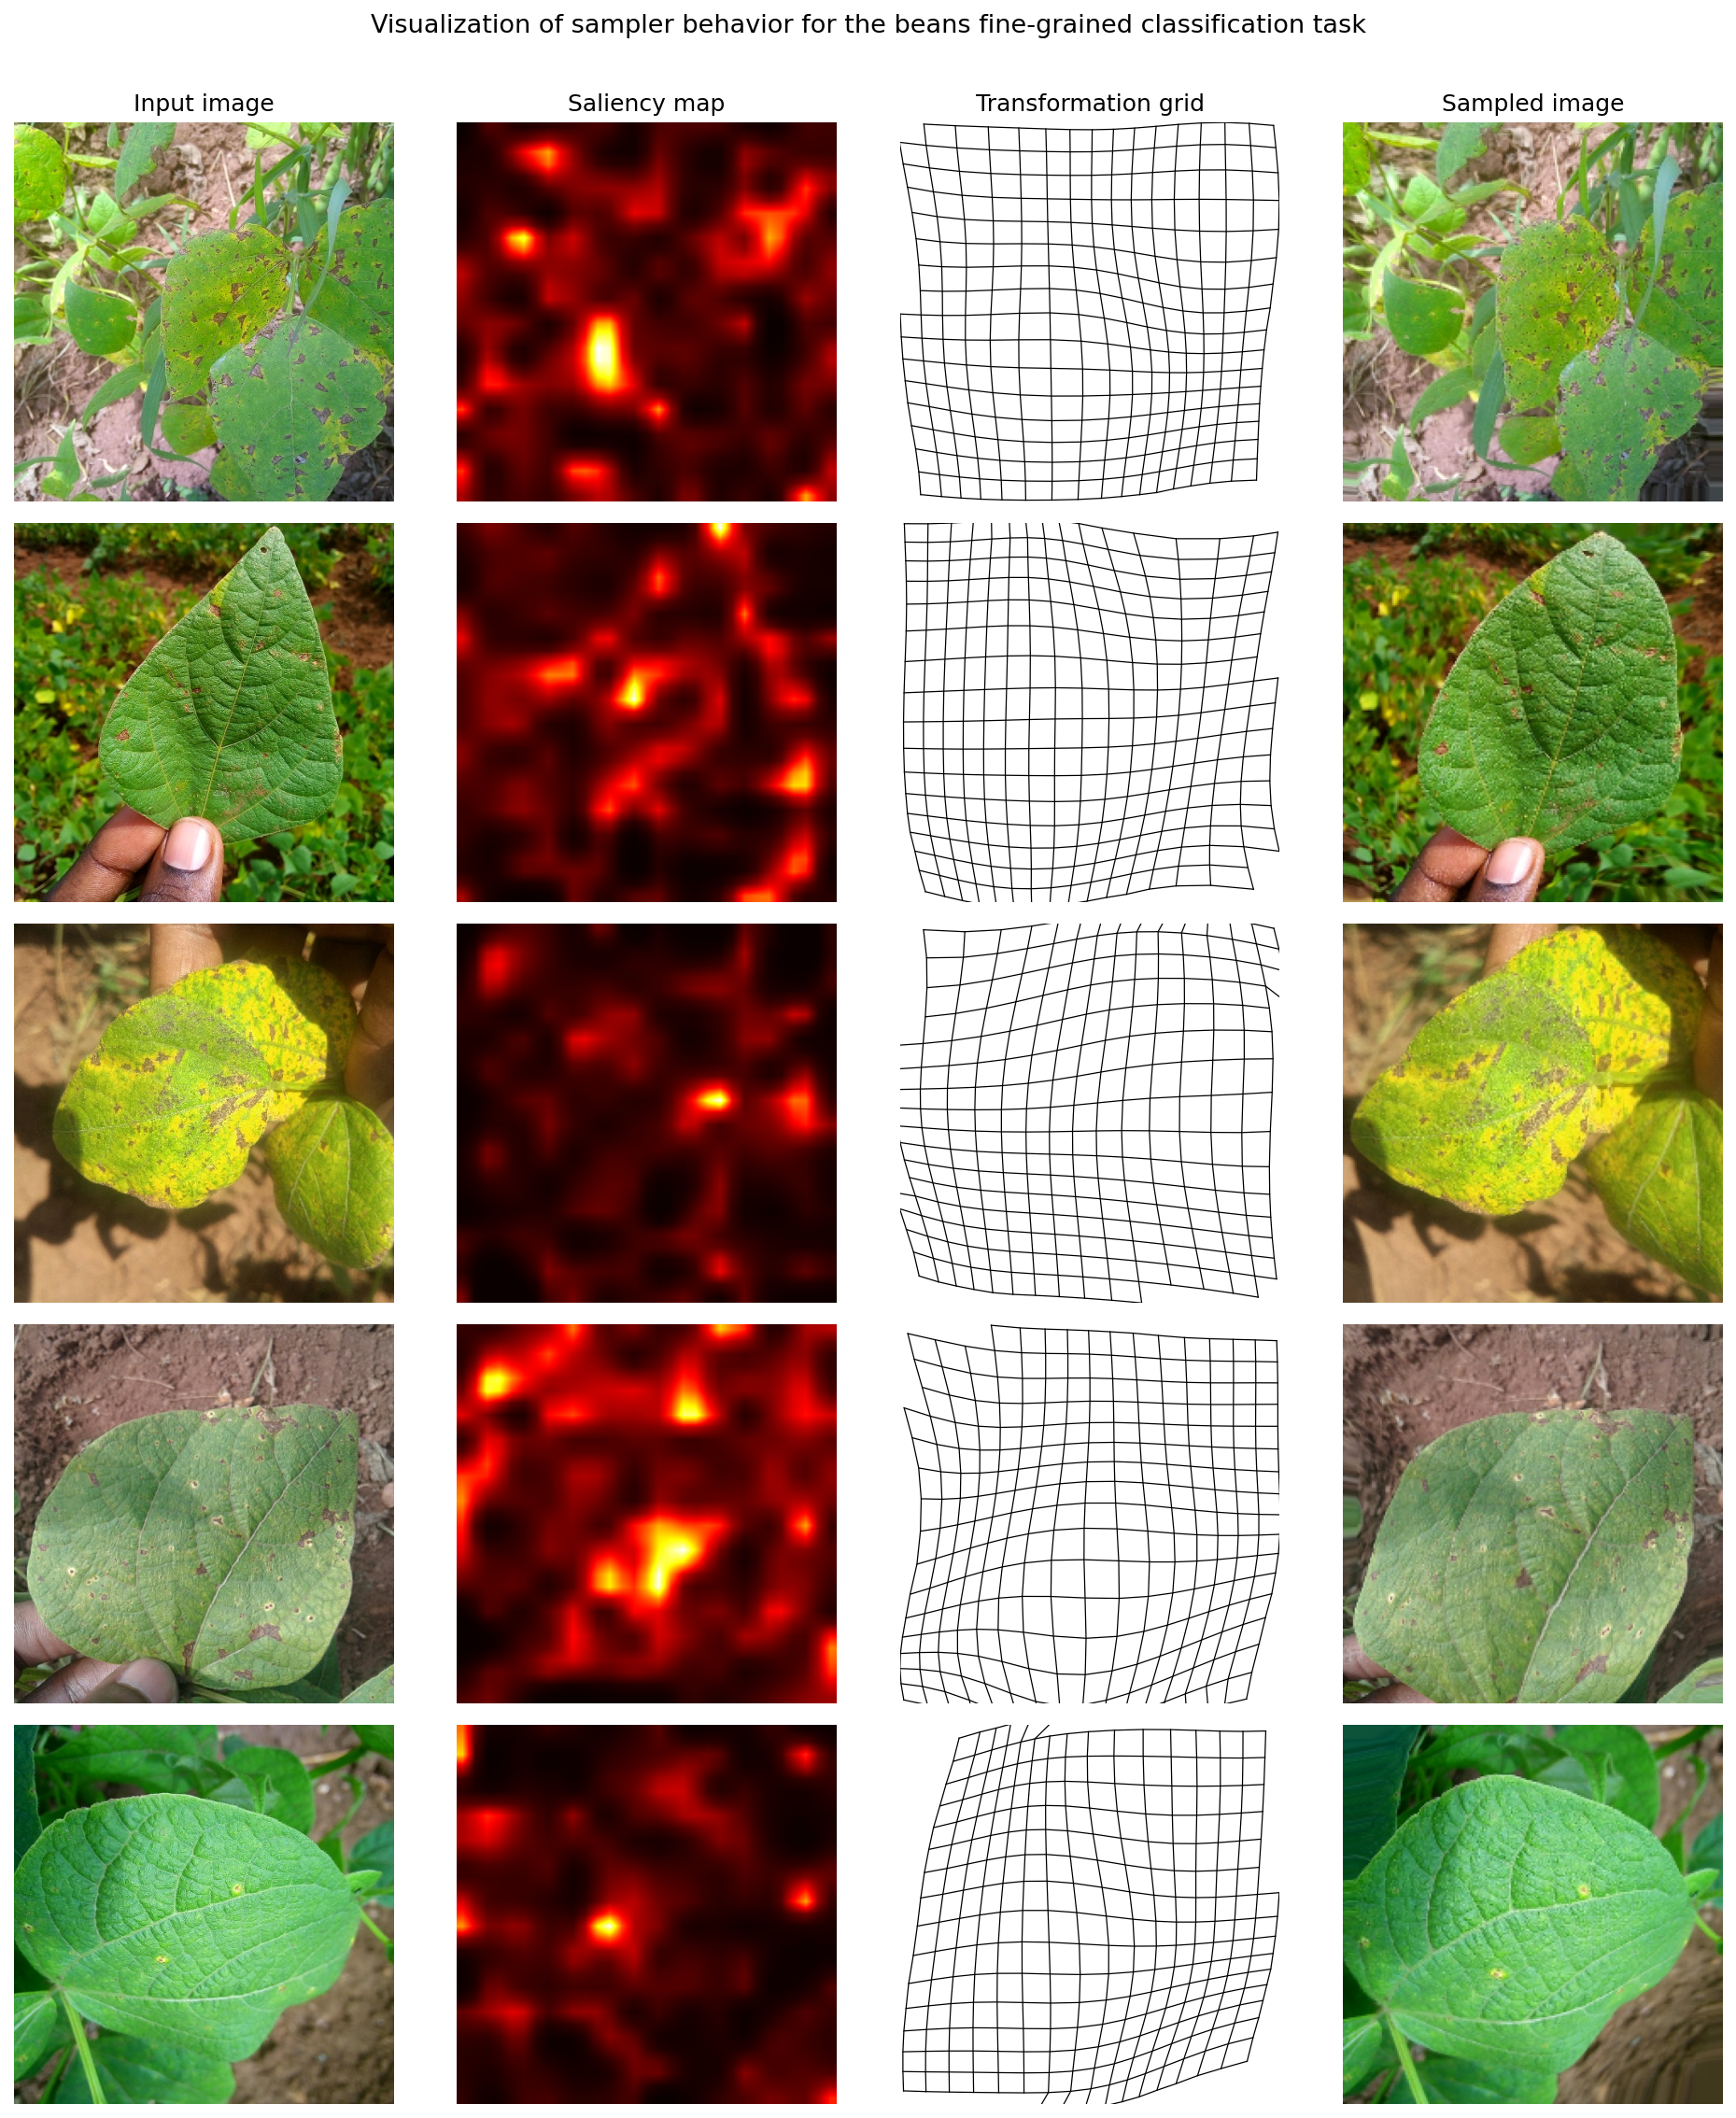
\includegraphics[width=0.95\linewidth]{../Figures/sampler_final.png}
\caption{Visualization of sampler behavior for the beans fine-grained
classification task.  For each test image (rows), the columns show the
original input, the saliency map produced by the trained $f_{s}$, the
deformation grid in output coordinates, and the resulting warped image
fed to the student.  The saliency network discovers and zooms in on
small lesion-like regions of the leaf.}
\label{fig:sampler_qualitative}
\end{figure}

% ============================================================
\section{Conclusion}
% ============================================================
We distil a $85.8$\,M-parameter ViT-B/16 teacher fine-tuned on the
\emph{beans} leaf-disease dataset into a $2.23$\,M-parameter MobileNetV2
student.  Random-init distillation (Table~\ref{tab:test_results}) lifts
the student by $+10.9$ accuracy points over the no-distillation
baseline, but the largest contributor to absolute performance is in fact
ImageNet-1k initialization, which alone closes most of the
baseline-to-teacher gap (Table~\ref{tab:test_results_imagenet}).
Plugging the saliency sampler of \cite{recasens2018learning} in front of
the ImageNet-initialized student
(Section~\ref{subsec:sampler_results}) preserves fine-grained lesion
detail and yields a final test accuracy of $0.9766$ with macro-F1
$0.9767$, exceeding the ViT teacher by $+0.039$ points while using only
$2.8\%$ of its parameters.  An ablation isolates distillation as the
decisive ingredient under the sampler ($+0.078$ points over the no-KD
control at the same validation accuracy).  These results are based on a
single seed and a small test split ($N{=}128$); we expect that
multi-seed evaluation, the larger Mugalu \emph{et~al.}~beans
release~\cite{mugalu2022makerere}, and a deployment-side latency study
on edge devices would give a fuller picture of the trade-offs.

% ============================================================
\bibliographystyle{plain}
\bibliography{references}
% ============================================================

\end{document}
